% Provenance (never printed): see sources/outline_sources.md (Year 3: refraction and
% reflection seismic methods; CMP acquisition, NMO, stacking, Dix; migration in
% principle; seismic stratigraphy). Brief: sources/book5/BRIEFS.md, ch. 2. Curves from
% figdata/bachelor-3/seismic_model.py, refraction_dip.py, synthetic_seismogram.py,
% cmp_nmo.py (the Varden column, region.py); exercise and problem values in the
% Book 5 scratch calculator calc/ch02.py.
\chapter{علم الزلازل الاستكشافي}\label{ch:b3:exploration-seismology}

تسير سفينة مسح ببطء على خط مستقيم في البحر، تجرّ مصفوفة من
مدافع الهواء على عمق بضعة أمتار تحت السطح، وخلفها كابلات طولها عدّة
كيلومترات مزوّدة بمسامع مائية. وفي أحد المسوح الموصوفة للهيئة التنظيمية،
احتوت المصفوفة على \num{5240} بوصة مكعّبة من الهواء المضغوط، وكانت تُطلق كلّ
\qty{8}{s} من عمق \qty{12}{m} تحت السطح، والكابلات الممتدّة ضيّقة السمت
خلف هذه السفن تسجّل الإزاحات من 8 إلى \qty{10}{km}.
% ledger: noaa5:wg-survey
كلّ طلقة ترسل نبضة صوتية إلى قاع البحر، وتعيد كلّ واجهة صخرية
تحتها صدى خافتًا. وبعد أسابيع من المعالجة، يتصفّح الجيولوجي
مقطعًا عرضيًا تظهر فيه قنوات الأنهار المدفونة والكتل الصدعية المائلة،
والحشوة ذات \omterm{def:b3:exploration-seismology:terminations}{التراكب الصاعد} لحوض قديم، كأنّما الأرض قد شُقّت فانكشفت.
استخدم علم الزلازل على نطاق الأرض في الفصل السابق أمواج
الزلازل؛ أمّا علم الزلازل الاستكشافي فيُنتج أمواجه الخاصّة، بمصادر يُعرف
زمنها ومكانها بدقّة، ويسجّلها على آلاف القنوات. يتتبّع هذا
الفصل الأصداء من الطلقة حتى المقطع: المسوح الزلزالية الانكسارية،
انعكاس \omterm{def:b3:exploration-seismology:wavelet}{الموجة الزلزالية القصيرة} عن عمود طبقي، وطريقة \omterm{def:b3:exploration-seismology:cmp}{نقطة المنتصف المشتركة}
التي تحوّل الأصداء المتكرّرة إلى سرعات وصورة نظيفة، والترحيل، الذي
يعيد العواكس إلى مواضعها الصحيحة، وقراءة المقطع بوصفه
ستراتيغرافيا.

\begin{recall}
عند الحدّ الفاصل بين وسطين ذوي ممانعة صوتية $Z_1 = \rho_1v_1$
و$Z_2 = \rho_2v_2$، تنعكس موجة مستوية عند السقوط العمودي بمعامل السعة
$R = (Z_2 - Z_1)/(Z_2 + Z_1)$ (من كتب الفيزياء، مجلد السنة الثانية
عن الموجات عند الواجهات). تُدرس موجة الرأس وزمن القطع ومسافة التقاطع
لمقطع انكساري فوق طبقات مستوية فقد دُرست في
مجلد السنة الأولى، في فصلها عن الأرض ذات الطبقات؛ وسجلات الآبار في الكتاب 2
(الصف 11). الالتفاف $(f*g)(t) = \int f(\tau)g(t - \tau)\,\mathrm d\tau$
وتحويل فورييه من كتب الرياضيات. أمّا \omterm{def:b3:seismology-imaging:ray-parameter}{معامل الشعاع} \omterm{def:b3:seismology-imaging:inverse}{والمسألة العكسية} الخطية
فهما المذكوران في \cref{ch:b3:seismology-imaging}.
\end{recall}

\section{المسوح الزلزالية الانكسارية}

\begin{definition}[المسح الزلزالي الانكساري والانعكاسي]\label{def:b3:exploration-seismology:surveys}
\emph{المسح الزلزالي الانكساري}\index{المسح الزلزالي الانكساري} يسجّل، على طول
خطّ من المستقبِلات أوائلَ الوصولات الصادرة عن مصدر مضبوط، ويستخدم
موجات الرأس التي تسري على قمّة الطبقات الأسرع لتحديد سرعاتها
وأعماقها. \emph{المسح الزلزالي الانعكاسي}\index{المسح الزلزالي الانعكاسي} يسجّل
كامل قطار الموجات، عند إزاحات تقلّ في الغالب عن الأعماق محلّ الاهتمام،
ويستخدم الموجات المنعكسة عن الواجهات عند سقوط قريب من العمودي
لتصوير التطبّق.
\end{definition}

فوق الطبقات المستوية تصل موجة الرأس عند $t = x/v_2 + t_i$، وهو خطّ مستقيم
يُعطي ميله سرعة $v_2$ للطبقة المنكسرة، ويُعطي قطعه $t_i$
عمقها. الطبقة المنكسرة المائلة تُميل الخطّ: موجة الرأس المطلقة باتجاه الانحدار
تصل متأخّرة أكثر فأكثر كلّما ازدادت الطبقة عمقًا، فتبدو بطيئة؛
أمّا المطلقة عكس اتجاه الانحدار فتبدو سريعة. ولو أُطلقت من الطرفين على الخطّ نفسه،
أي في مقطع معكوس، فإنّه يفصل السرعة عن الانحدار.

\begin{theorem}[الانكسار على واجهة مائلة]\label{thm:b3:exploration-seismology:dipping}
طبقة سرعتها $v_1$ تعلو طبقةً منكسرةً مستويةً سرعتها $v_2 > v_1$ ومائلةً
بالزاوية $\theta$ على امتداد المقطع؛ $i_c = \arcsin(v_1/v_2)$، و$h$ هو
العمق العمودي للطبقة المنكسرة تحت الطلقة. وبعد المسافة الحرجة
تصل موجة الرأس عند
\begin{align*}
  t &= \frac{x\sin(i_c + \theta)}{v_1} + \frac{2h\cos i_c}{v_1}
  &&\text{الإطلاق مع اتجاه الانحدار},\\
  t &= \frac{x\sin(i_c - \theta)}{v_1} + \frac{2h\cos i_c}{v_1}
  &&\text{الإطلاق عكس اتجاه الانحدار}.
\end{align*}
السرعتان الظاهريتان لمقطع معكوس، $v_d = v_1/\sin(i_c + \theta)$
و$v_u = v_1/\sin(i_c - \theta)$ تُعطيان
\[
  i_c = \tfrac12\left[\arcsin\frac{v_1}{v_d} + \arcsin\frac{v_1}{v_u}\right],\qquad
  \theta = \tfrac12\left[\arcsin\frac{v_1}{v_d} - \arcsin\frac{v_1}{v_u}\right],
  \qquad v_2 = \frac{v_1}{\sin i_c} .
\]
\end{theorem}

\begin{proof}
نُدوِّر الإطار بحيث تصبح الطبقة المنكسرة أفقية؛ فيميل السطح حينئذ
بالزاوية $\theta$، وعند الإطلاق باتجاه الانحدار يكون العمق العمودي تحت مستقبِل عند الإزاحة
$x$ هو $h + x\sin\theta$، وإسقاطه على الطبقة المنكسرة
$x\cos\theta$. يهبط مسار موجة الرأس بالزاوية الحرجة $i_c$ حتى
العمودي، ثم يسير على امتداد الطبقة المنكسرة بالسرعة $v_2$ ويصعد بالزاوية $i_c$. ويكون زمنه
\[
  t = \frac{h}{v_1\cos i_c} + \frac{x\cos\theta - h\tan i_c - (h + x\sin\theta)\tan i_c}{v_2}
  + \frac{h + x\sin\theta}{v_1\cos i_c}.
\]
باعتماد $1/v_2 = \sin i_c/v_1$ و$1/\cos i_c - \sin i_c\tan i_c = \cos i_c$،
فتُعطي الحدود ذات $h$ القيمة $2h\cos i_c/v_1$، وتُعطي الحدود ذات $x$
$x(\sin i_c\cos\theta + \cos i_c\sin\theta)/v_1 = x\sin(i_c + \theta)/v_1$.
عند الإطلاق عكس اتجاه الانحدار تتغيّر إشارة $\theta$. وتُعكس الصيغ الأخيرة
السرعتين الظاهريتين.
\end{proof}

يجب أن يُعطي فرعا المقطع المعكوس الزمنَ نفسه بين نقطتي الإطلاق،
أيّ الطرفين أُطلق: \emph{الزمن المتبادل}، وهو تحقّق من
قراءة الأوائل. ويُبطل الطريقةَ موقفان. طبقةٌ أبطأ من التي تعلوها
(قلب السرعة) لا تُنتج موجة رأس فتبقى غير مرئية: تُحسب صخورها
ضمن الطبقة التي فوقها، وتُقدَّر كلّ الأعماق التي تحتها بأكثر من قيمتها.
وطبقةٌ أسرع من التي فوقها لكنّها رقيقة جدًّا قد لا تُعطي وصولًا أوّلًا أبدًا، لأنّ
موجة الرأس للطبقة الأعمق والأسرع تتجاوزها: طبقة مخفيّة. أمّا
المسح الانعكاسي فيرصد الحالتين.

\begin{omfigure}
\begin{tikzpicture}
\begin{axis}[omrecord, width=0.82\linewidth, height=0.46\linewidth,
  xmin=0, xmax=1200, ymin=0, ymax=660,
  xlabel={الموضع على امتداد المصفوفة، من الطلقة الغربية \babelsublr{(\unit{m})}},
  ylabel={الزمن \babelsublr{(\unit{ms})}}, legend pos=north west, legend cell align=left,
  legend style={font=\scriptsize}]
\addplot[gray, thick, densely dashed] table[x=x, y=tdir] {figdata/out/bachelor-3-refraction_dip-west.dat};
\addlegendentry{\foreignlanguage{arabic}{الموجات المباشرة ($v_1$)}}
\addplot[blue!70!black, thick] table[x=x, y=thead] {figdata/out/bachelor-3-refraction_dip-west.dat};
\addlegendentry{موجة الرأس من الغرب، مطلقة عكس اتجاه الانحدار}
\addplot[red!70!black, thick] table[x expr=1200-\thisrow{x}, y=thead] {figdata/out/bachelor-3-refraction_dip-east.dat};
\addlegendentry{موجة الرأس من الشرق، مطلقة باتجاه الانحدار}
\addplot[gray, thick, densely dashed, forget plot] table[x expr=1200-\thisrow{x}, y=tdir] {figdata/out/bachelor-3-refraction_dip-east.dat};
\addplot[only marks, mark=*, mark size=1.5pt] coordinates {(1200,486.13) (0,486.13)};
\node[font=\scriptsize, anchor=south east] at (axis cs:1190,530) {الزمن المتبادل};
\end{axis}
\end{tikzpicture}

\par\smallskip{\small مقطع انكسار زلزالي معكوس على الجناح الغربي
للطية المحدبة لفاردن (محسوب؛ مسألة، الجزء الأول). الطبقة المنكسِرة، أي قمّة
الحجر الجيري، يرتفع من الغرب إلى الشرق بزاوية \ang{10.8} تحت امتداد \qty{1200}{m}؛
الطباشير والطَّفل فوقه مُجمَّعان في طبقة واحدة سرعتها \qty{2.40}{km.s^{-1}}. أمّا
موجة الرأس المطلقة من الغرب عكس اتجاه الانحدار تبدو سريعة (\qty{6.57}{km.s^{-1}})، والمطلقة
من الشرق باتجاه الانحدار بطيئة (\qty{3.52}{km.s^{-1}})؛ ويستغرق كلٌّ منهما \qty{486.1}{ms} لعبور
الامتداد كلّه. لا تلحق موجات الرأس بالموجات المباشرة إلّا قرب
الطرف البعيد: الطبقة المنكسِرة عميقة لامتداد قصير إلى هذا الحد.}
\label{fig:b3:exploration-seismology:refraction}
\end{omfigure}

\section{الانعكاس عند الورود العمودي}

\begin{definition}[الموجة الزلزالية القصيرة، موجة ريكر القصيرة]\label{def:b3:exploration-seismology:wavelet}
\emph{الموجة الزلزالية القصيرة}\index{الموجة الزلزالية القصيرة} هي النبضة القصيرة التي تدوم بضعة عشرات
من الميلي ثانية، يرسلها المصدر ونظام التسجيل عبر
الأرض؛ يُعيد كلُّ عاكس نسخةً مُحجَّمةً منها. و\emph{موجة ريكر
القصيرة}\index{موجة ريكر القصيرة} ذات التردد الذروي $f$ هي النبضة ذات الطور الصفري
\[
  w(t) = \left(1 - 2\pi^2f^2t^2\right)e^{-\pi^2f^2t^2},
\]
وهي المشتقّة الثانية لدالة غاوس، باستثناء الإشارة والمقياس: ذروة مركزية
وفصّان جانبيان، ومتوسطها صفر، وطيف سعتها يبلغ ذروته عند $f$.
\end{definition}

\begin{definition}[متسلسلة الانعكاسية]\label{def:b3:exploration-seismology:synthetic}
\emph{متسلسلة الانعكاسية}\index{متسلسلة الانعكاسية} لعمود طبقي هي
المتتالية من معاملات الانعكاس عند الورود العمودي $r_k$ لسطوحها البينية،
موضوعةً عند أزمنتها الرأسية ذهابًا وإيابًا $\tau_k = \sum_{i \le k} 2h_i/v_i$:
$r(t) = \sum_k r_k\,\delta(t - \tau_k)$.
\end{definition}

\begin{proposition}[النموذج الالتفافي]\label{prop:b3:exploration-seismology:synthetic}
إذا اقتصرنا على الانعكاسات الأولية وحدها (دون المتعدّدة)، عند الورود العمودي، مع
غياب فقد النفاذ والتوهين والانتشار، وكانت الموجة القصيرة $w$ لا
تتغيّر مع العمق، فإنّ الأثر المسجَّل هو التفاف الموجة القصيرة مع
\omterm{def:b3:exploration-seismology:synthetic}{متسلسلة الانعكاسية}:
\[
  s(t) = \sum_k r_k\,w(t - \tau_k) = (w*r)(t) .
\]
الأثر المحسوب بهذه الطريقة من سجل ثقب الحفر للسرعة والكثافة هو
\emph{المخطط الزلزالي الاصطناعي}\index{المخطط الزلزالي الاصطناعي} لهذا السجل.
\end{proposition}

\begin{proof}
يُعيد كلُّ سطح بيني نسخةً من الموجة الساقطة مُحجَّمةً بمعامله
ومتأخّرةً بزمن ذهابه وإيابه؛ والتسجيل خطّي، فتتراكم النسخ.
والمجموع هو التفاف $w$ مع قطار النبضات الديراكية الموزونة
$r(t)$، لأنّ $w*\delta(\cdot - \tau_k) = w(\cdot - \tau_k)$.
\end{proof}

\omterm{prop:b3:exploration-seismology:synthetic}{المخطط الزلزالي الاصطناعي} هو الوسيلة التي يُربط بها ثقب الحفر بالمقطع الزلزالي:
يُطابَق انعكاسٌ على المقطع مع السطح البيني في السجل الذي يُنتجه.
يقع عمود فاردن الطبقي أسفل محور الطية المقعرة في المسألة (النموذج الزلزالي
لهذا الفصل، مع سرعات وكثافات مختارة ضمن المديات المنشورة
لكلّ صخرة)
% ledger: mavko:velocities
يُعطي الشكل أدناه. لا يعكس السطح البيني بين الطباشير والطَّفل إلّا
\qty{2.8}{\percent} من السعة، لأنّ الطباشير والطَّفل يصادف أن يكون لهما
معاوقةٌ متقاربة جدًّا؛ أمّا قمة الحجر الجيري فتعكس \qty{38}{\percent}،
وقاعدة الحجر الجيري تُعيد نبضةً معكوسة، والأساس الصخري نبضةً
موجبةً قويةً.

\begin{omfigure}
\begin{tikzpicture}
\begin{groupplot}[group style={group size=3 by 1, horizontal sep=0.45cm, y descriptions at=edge left},
  width=0.36\linewidth, height=0.6\linewidth, y dir=reverse, ymin=0.4, ymax=0.85,
  tick label style={font=\scriptsize}, label style={font=\small}, title style={font=\small}]
\nextgroupplot[title={المعاوقة}, xlabel={\mbox{\textdir TLT \scriptsize $10^6$\,\unit{kg.m^{-2}.s^{-1}}}},
  ylabel={زمن الذهاب والإياب \babelsublr{(\unit{s})}}, xmin=4, xmax=14]
\addplot[black, thick] table[x=imp, y=t] {figdata/out/bachelor-3-synthetic_seismogram-log.dat};
\node[font=\tiny, anchor=west] at (axis cs:5.1,0.45) {الطباشير};
\node[font=\tiny, anchor=west] at (axis cs:5.4,0.535) {الطَّفل};
\node[font=\tiny, anchor=east] at (axis cs:11.6,0.62) {الحجر الجيري};
\node[font=\tiny, anchor=west] at (axis cs:7.0,0.70) {الحجر الرملي};
\node[font=\tiny, anchor=east] at (axis cs:13.1,0.79) {الشيست};
\nextgroupplot[title={الانعكاسية}, xmin=-0.45, xmax=0.45, xtick={-0.4,0,0.4}]
\addplot[xcomb, red!70!black, thick, mark=*, mark size=1.2pt] table[x=r, y=t] {figdata/out/bachelor-3-synthetic_seismogram-refl.dat};
\draw[gray] (axis cs:0,0.4) -- (axis cs:0,0.85);
\nextgroupplot[title={الأثر الاصطناعي}, xmin=-0.45, xmax=0.45, xtick={-0.4,0,0.4}]
\addplot[blue!70!black, thick] table[x=s, y=t] {figdata/out/bachelor-3-synthetic_seismogram-trace.dat};
\draw[gray] (axis cs:0,0.4) -- (axis cs:0,0.85);
\end{groupplot}
\end{tikzpicture}

\par\smallskip{\small \omterm{prop:b3:exploration-seismology:synthetic}{المخطط الزلزالي الاصطناعي} لعمود فاردن الطبقي أسفل
محور الطية المقعرة (محسوب). يسارًا: المعاوقة لكلّ طبقة مقابل الزمن
ذهابًا وإيابًا. وسطًا: \omterm{def:b3:exploration-seismology:synthetic}{متسلسلة الانعكاسية}، بقمّة واحدة لكلّ سطح بيني (تشير الأعمدة
إلى اليمين عند زيادة المعاوقة). يمينًا: التفاف هذه المتسلسلة مع
\omterm{def:b3:exploration-seismology:wavelet}{موجة ريكر القصيرة} ذات التردد \qty{30}{Hz}. كلُّ انعكاس نسخةٌ من الموجة القصيرة؛ أمّا
الانعكاس الخافت بين الطباشير والطَّفل عند \qty{0.488}{s} فبالكاد يُرى.}
\label{fig:b3:exploration-seismology:synthetic}
\end{omfigure}

ما أرقّ طبقة يمكن للانعكاسات أن تفصلها؟ تُعيد قمّتها وقاعدتها كلٌّ منهما
موجةً قصيرة؛ فإذا تراكبتا تداخلتا.

\begin{definition}[سمك التوليف]\label{def:b3:exploration-seismology:resolution}
\emph{سمك التوليف}\index{سمك التوليف} لطبقة ما هو السمك
الذي تتداخل عنده الانعكاسات الآتية من قمّتها وقاعدتها، المختلفة في الإشارة،
تداخلًا بنّاءً أكبر ما يمكن، فتبلغ السعة المركّبة أعلى قيمة لها. أمّا الطبقات الأرقّ
فلا يمكن فصلها: إذ لم تعد قمّتها وقاعدتها قابلتين للتعيين كلٌّ على حدة،
وتتناقص السعةُ تناسبًا مع السمك.
\end{definition}

\begin{proposition}[قاعدة ربع الطول الموجي]\label{prop:b3:exploration-seismology:tuning}
لموجة قصيرة دورها السائد $T$ في طبقة سرعتها $v$، ومعاملا الانعكاس
$+R$ عند قمّتها و$-R$ عند قاعدتها، فإنّ الانعكاس المركّب يكون
أقوى ما يكون عندما يكون سمك الطبقة $b = \lambda/4$، حيث $\lambda = vT$؛ ومن أجل
$b \ll \lambda/4$ تكون سعته متناسبة طرديًّا مع $b$.
\end{proposition}

\begin{proof}
نمثّل الموجة القصيرة بتوافقيّها السائد $\cos(2\pi t/T)$. والانعكاسان
هما $R\cos(2\pi t/T) - R\cos(2\pi(t - \Delta t)/T)$ حيث
$\Delta t = 2b/v$، وتكون سعته $2R|\sin(\pi\Delta t/T)|$ أكبر ما يكون عندما
$\Delta t = T/2$، أي $b = vT/4$؛ ومن أجل $\Delta t$ الصغيرة تكون تقريبًا
$2\pi R\Delta t/T = 4\pi Rb/\lambda$.
\end{proof}

ليست موجةُ ريكر القصيرة توافقيةً، وسمكُ توليفها، المقروءُ من نموذج الإسفين
في الشكل أدناه، أصغرُ قليلًا من ربع الطول الموجي
عند تردّد الذروة: \qty{19.5}{m} عند \qty{30}{Hz} في صخر سرعته
\qty{3000}{m.s^{-1}}، إذ $\lambda/4 = \qty{25}{m}$. نادرًا ما تحتوي البيانات الزلزالية
طاقةً كبيرة فوق بضعة عشرات من الهرتز قادمةً من أعماق بالكيلومترات، لأنّ
الصخور تمتصّ الترددات العالية؛ وتُرى الطبقات التي يقلّ سمكها عن نحو \qty{20}{m}
انعكاسًا مفردًا.

\begin{omfigure}
\begin{tikzpicture}
\begin{axis}[omrecord, width=0.74\linewidth, height=0.42\linewidth,
  xmin=0, xmax=80, ymin=0, ymax=1.8,
  xlabel={سمك الطبقة $b$ \babelsublr{(\unit{m})}}, ylabel={السعة القصوى / $R$}]
\addplot[blue!70!black, thick] table[x=b, y expr=2*\thisrow{amp}] {figdata/out/bachelor-3-synthetic_seismogram-wedge.dat};
\draw[red!70!black, densely dashed] (axis cs:19.5,0) -- (axis cs:19.5,1.6);
\node[font=\scriptsize, anchor=south, red!70!black] at (axis cs:19.5,1.6) {\foreignlanguage{arabic}{التوليف، \mbox{\textdir TLT \qty{19.5}{m}}}};
\draw[gray, densely dotted] (axis cs:25,0) -- (axis cs:25,1.6);
\node[font=\scriptsize, anchor=west, gray!40!black] at (axis cs:25.5,0.3) {$\lambda/4 = \qty{25}{m}$};
\draw[gray] (axis cs:0,1) -- (axis cs:80,1);
\node[font=\scriptsize, anchor=south east] at (axis cs:79,1) {موجتان منفصلتان};
\end{axis}
\end{tikzpicture}

\par\smallskip{\small نموذج الإسفين (محسوب): طبقة سرعتها
\qty{3000}{m.s^{-1}} ومعاملا الانعكاس $+R$ عند قمّتها و$-R$ عند
قاعدتها، مُصوَّرةً \omterm{def:b3:exploration-seismology:wavelet}{بموجة ريكر القصيرة} \qty{30}{Hz}. أمّا السعة القصوى للانعكاس المركّب، بالنسبة إلى انعكاس مفرد معامله $R$،
فتتزايد خطيًّا من الصفر في الطبقات الرقيقة جدًّا،
وتبلغ ذروتها عند \omterm{def:b3:exploration-seismology:resolution}{سمك التوليف}، وتستقرّ عند مستوى موجتين منفصلتين
في الطبقات السميكة.}
\label{fig:b3:exploration-seismology:wedge}
\end{omfigure}

وفي الاتجاه الجانبي يتحدّد الوضوح بعرض العاكس الذي يُعيد
الطاقةَ في الطور نفسه.

\begin{definition}[نطاق فرينل]\label{def:b3:exploration-seismology:fresnel}
\emph{نطاق فرينل}\index{نطاق فرينل} (الأوّل) لعاكسٍ، عند مصدر ومستقبل متطابقين
على ارتفاع $z$ فوقه، هو قرصٌ من العاكس يحيط بنقطة السقوط العمودي، يكون فيه
المسار المزدوج أطول من المسار العادي بأقلّ من نصف طول موجي،
فتصل انعكاساته في الطور نفسه،
وتُكوِّن معًا الانعكاسَ المسجَّل.
\end{definition}

\begin{proposition}[نصف قطر نطاق فرينل]\label{prop:b3:exploration-seismology:fresnel}
يكون \omterm{def:b3:exploration-seismology:fresnel}{لنطاق فرينل} الأوّل نصف القطر
$r_F = \sqrt{\lambda z/2 + \lambda^2/16} \approx \sqrt{\lambda z/2}$ من أجل
$\lambda \ll z$.
\end{proposition}

\begin{proof}
تقع نقطة من العاكس على بُعد $r$ من نقطة السقوط العمودي
على بُعد $\sqrt{z^2 + r^2}$ من المصدر. ويكون فائض المسار المزدوج
$2(\sqrt{z^2 + r^2} - z)$؛ وبجعله يساوي $\lambda/2$ نجد
$\sqrt{z^2 + r^2} = z + \lambda/4$، ومنه $r^2 = \lambda z/2 + \lambda^2/16$.
\end{proof}

عند عمق \qty{1}{km}، ومع $\lambda = \qty{100}{m}$، يبلغ نصف قطر \omterm{def:b3:exploration-seismology:fresnel}{نطاق فرينل}
\qty{225}{m} تقريبًا: فالتفاصيل الأضيق من ذلك تُطمس، ما لم
يضغط الترحيلُ (أدناه) هذا النطاق.

\begin{omfigure}
\begin{tikzpicture}[font=\small, x=1cm, y=1cm]
\fill[brown!12] (-4.5,-3.6) rectangle (4.5,-3.0);
\draw[thick] (-4.5,-3.0) -- (4.5,-3.0);
\node[anchor=north west] at (-4.4,-3.05) {عاكس};
\draw[thick] (-4.5,0) -- (4.5,0);
\fill (0,0) circle (2.2pt) node[above] {مصدر ومستقبل};
\draw[->, thick] (0,0) -- (0,-2.97);
\node[anchor=west] at (0.05,-1.5) {$z$};
\draw[blue!70!black, thick] (0,0) -- (1.9,-3.0);
\draw[blue!70!black, thick] (0,0) -- (-1.9,-3.0);
\node[anchor=west, blue!70!black] at (1.0,-1.2) {$z + \lambda/4$};
\fill[red!25, opacity=0.7] (-1.9,-3.08) rectangle (1.9,-2.92);
\draw[red!70!black] (0,-3.65) -- (0,-3.95) (1.9,-3.1) -- (1.9,-3.95);
\draw[<->, red!70!black] (0,-3.85) -- (1.9,-3.85) node[midway, below] {$r_F$};
\draw[gray, densely dashed] (-57.6:3.55) arc (-57.6:-122.4:3.55);
\end{tikzpicture}

\par\smallskip{\small \omterm{def:b3:exploration-seismology:fresnel}{نطاق فرينل} الأوّل (تخطيطي): الجزء من العاكس
الذي تتجاوز مسافتُه من مصدر ومستقبل متطابقين المسافةَ العمودية $z$
بأقلّ من $\lambda/4$ (القوس المتقطّع: الكرة ذات نصف القطر
$z + \lambda/4$)، بحيث يكون فائض المسار المزدوج أقلّ من نصف طول موجي،
فتصل أصداؤه في الطور نفسه. وقد جرى تضخيم مقياس $\lambda$.}
\label{fig:b3:exploration-seismology:fresnel}
\end{omfigure}

\section{الحصول على نقطة المنتصف المشتركة ومعالجتها}

لا يُرى الصدى المفرد بوضوح وسط الضجيج، لذلك تسجّل مسوح الانعكاس
كلّ نقطة تحت السطح مرّات عديدة، بأزواج مختلفة من المصادر والمستقبلات،
وتجمع التسجيلات.

\begin{definition}[نقطة المنتصف المشتركة، تعدّدية التغطية]\label{def:b3:exploration-seismology:cmp}
لمصدرٍ عند $x_s$ ومستقبلٍ عند $x_r$ على خطّ، فإنّ المنتصف هو
$(x_s + x_r)/2$ والإزاحة $x = |x_r - x_s|$. مجموعةُ \emph{نقطة
المنتصف المشتركة}\index{نقطة المنتصف المشتركة} (CMP) هي مجموعة الآثار، من جميع الطلقات، التي تشترك في المنتصف نفسه؛
وفوق طبقات أفقية تنعكس كلّها من النقطة
نفسها تحت السطح. أمّا \emph{تعدّدية التغطية}\index{تعدّدية التغطية}
فهي عدد الآثار في المجموعة. ومع $N$ قنوات عند
فاصل المستقبِلات $\Delta g$ وطلقةٍ كلّ $\Delta s$ على امتداد الخطّ، تكون
التعدّدية $N\Delta g/(2\Delta s)$.
\end{definition}

\begin{omfigure}
\begin{tikzpicture}[font=\small, x=1cm, y=1cm]
\draw[thick] (-5,0) -- (5,0);
\fill[brown!10] (-5,-2.6) rectangle (5,-2.2);
\draw[thick] (-5,-2.2) -- (5,-2.2);
 \node[anchor=north east] at (5,-2.25) {العاكس};
\foreach \off/\col in {0.8/blue!70!black, 2.0/red!70!black, 3.4/green!45!black, 4.6/orange!80!black} {
  \draw[\col, thick] (-\off,0) -- (0,-2.2) -- (\off,0);
  \fill[\col] (-\off,0) circle (2.4pt);
  \fill[\col] (\off-0.12,0) -- (\off+0.12,0) -- (\off,0.2) -- cycle;
}
\fill (0,-2.2) circle (2pt);
\draw[densely dashed] (0,0.6) -- (0,-2.2);
 \node[anchor=south] at (0,0.6) {نقطة المنتصف المشتركة};
 \node[anchor=north, align=center, font=\scriptsize] at (0,-2.65) {\foreignlanguage{arabic}{نقطة العمق المشتركة (العاكس المستوي)}};
 \node[anchor=south, font=\scriptsize] at (-4.6,0.08) {الطلقات};
 \node[anchor=south, font=\scriptsize] at (4.6,0.25) {المستقبِلات};
\end{tikzpicture}

\par\smallskip{\small هندسة \omterm{def:b3:exploration-seismology:cmp}{نقطة المنتصف المشتركة} (تخطيطية): أربعة أزواج من المصدر--المستقبِل
(نقاط، مثلثات) ذات إزاحات مختلفة تشترك في المنتصف نفسه؛ فوق
عاكس مستوٍ تنعكس جميعها من النقطة نفسها أسفله. وتكوّن آثارها
مجموعةً تعدّديتها أربعة.}
\label{fig:b3:exploration-seismology:cmp}
\end{omfigure}

\begin{theorem}[الانزياح الزمني العادي]\label{thm:b3:exploration-seismology:nmo}
في طبقة سرعتها $v$ فوق عاكس مستوٍ عند الزمن الرأسي ذهابًا وإيابًا
$t_0$، فإنّ الانعكاس المسجَّل عند الإزاحة $x$ يصل إلى
\[
  t(x)^2 = t_0^2 + \frac{x^2}{v^2},
\]
قطعٌ زائد في المستوى $(x, t)$. والتأخّر $\Delta t = t(x) - t_0$ هو
\emph{الانزياح الزمني العادي}\index{الانزياح الزمني العادي}؛ ومن أجل $x \ll vt_0$،
$\Delta t \approx x^2/(2v^2t_0)$.
\end{theorem}

\begin{proof}
يمتد مسار الانعكاس من المصدر إلى نقطة الانعكاس تحت
المنتصف، ثم يعود صاعدًا إلى المستقبِل: ساقان طول كلٍّ منهما
$\sqrt{(vt_0/2)^2 + (x/2)^2}$. ومنه $t = (2/v)\sqrt{(vt_0/2)^2 + (x/2)^2}$
و$t^2 = t_0^2 + x^2/v^2$. ثمّ $t - t_0 = (t^2 - t_0^2)/(t + t_0) \approx
x^2/(2v^2t_0)$.
\end{proof}

فوق عدّة طبقات لم يعد زمن الانعكاس قطعًا زائدًا تمامًا، لكنّه
قريب منه تقريبًا عند الإزاحات الصغيرة، مع سرعة هي متوسط مرجَّح لسرعات
الطبقات.

\begin{definition}[التكديس، وسرعة الجذر التربيعي للمتوسط، والسرعة الفاصلية]\label{def:b3:exploration-seismology:velocities}
\emph{السرعة الفاصلية}\index{السرعة الفاصلية} $v_i$ للطبقة هي
سرعتها نفسها، ولِيكن $\Delta t_i = 2h_i/v_i$ الزمن ذهابًا وإيابًا عبرها، فإنّ
\emph{سرعة الجذر التربيعي للمتوسط}\index{سرعة الجذر التربيعي للمتوسط} حتى
قاع الطبقة $n$ هي
\[
  V_{\text{rms},n} = \left(\frac{\sum_{i\le n}v_i^2\,\Delta t_i}{\sum_{i\le n}\Delta t_i}\right)^{1/2}.
\]
\emph{سرعة التكديس}\index{سرعة التكديس} لانعكاسٍ هي
السرعة $V$ للقطع الزائد $t^2 = t_0^2 + x^2/V^2$ الذي يطابق أزمنته أفضل مطابقة في
مجموعة \omterm{def:b3:exploration-seismology:cmp}{نقطة المنتصف المشتركة}.
\end{definition}

\begin{proposition}[سرعة التكديس عند الإزاحات الصغيرة]\label{prop:b3:exploration-seismology:rms}
فوق طبقات أفقية، $t(x)^2 = t_0^2 + x^2/V_{\text{rms}}^2 + O(x^4)$: عند الإزاحات الصغيرة،
تكون \omterm{def:b3:exploration-seismology:velocities}{سرعة التكديس} هي \omterm{def:b3:exploration-seismology:velocities}{سرعة الجذر التربيعي للمتوسط}.
\end{proposition}

\begin{proof}
من أجل \omterm{def:b3:seismology-imaging:ray-parameter}{معامل الشعاع} $p$، يكون $x = \sum_i 2h_i\tan\varphi_i$
و$t = \sum_i 2h_i/(v_i\cos\varphi_i)$، مع $\sin\varphi_i = pv_i$. وحتى الرتبة الثانية
في $p$، $\tan\varphi_i \approx pv_i$ و$1/\cos\varphi_i \approx 1 +
p^2v_i^2/2$، فيكون $x \approx p\sum v_i^2\Delta t_i = pV_{\text{rms}}^2t_0$
و$t \approx t_0 + \tfrac12p^2V_{\text{rms}}^2t_0$. ثمّ
$t^2 \approx t_0^2 + p^2V_{\text{rms}}^2t_0^2 = t_0^2 + x^2/V_{\text{rms}}^2$، والحدود
المهملة من الرتبة $p^4$، أي $x^4$.
\end{proof}

\begin{theorem}[معادلة ديكس]\label{thm:b3:exploration-seismology:dix}
إذا كانت $V_{n-1}$ و$V_n$ سرعتي الجذر التربيعي للمتوسط حتى أعلى
الطبقة $n$ وقاعها، عند الزمنين ذهابًا وإيابًا $t_{n-1}$ و$t_n$، تُعطى \omterm{def:b3:exploration-seismology:velocities}{السرعة الفاصلية} للطبقة
وفق \emph{معادلة ديكس}\index{معادلة ديكس}
\[
  v_n^2 = \frac{V_n^2t_n - V_{n-1}^2t_{n-1}}{t_n - t_{n-1}} ,
\]
وسمكُها $h_n = v_n(t_n - t_{n-1})/2$.
\end{theorem}

\begin{proof}
بحسب التعريف، $V_n^2t_n = \sum_{i\le n}v_i^2\Delta t_i$ و$V_{n-1}^2t_{n-1}
= \sum_{i\le n-1}v_i^2\Delta t_i$. ويكون فرقهما $v_n^2\Delta t_n$، حيث
$\Delta t_n = t_n - t_{n-1}$.
\end{proof}

يفحص تحليلُ السرعة كلَّ مجموعة بحثًا عن القطع الزائد الذي يطابق أفضل ما يكون
الطاقة: من أجل كلّ $t_0$ و$V$، تُجمَع الآثار على امتداد المنحنى،
ويُرسَم مقياسٌ للتماسك يُسمّى التشابه؛ ويختار المحلِّل قممه،
عاكسًا فعاكسًا، لبناء دالة السرعة. ثمّ يُزيح تصحيحُ NMO
كلّ عيّنة من كلّ أثر من $t(x)$ إلى $t_0$، فتُسطَّح
الانعكاسات، وتُجمَع آثار كلّ مجموعة.

\begin{definition}[التكديس]\label{def:b3:exploration-seismology:stack}
\emph{التكديس}\index{التكديس} هو جمع آثار المجموعة، بعد
تصحيح \omterm{thm:b3:exploration-seismology:nmo}{الانزياح الزمني العادي}، لآثار مجموعة \omterm{def:b3:exploration-seismology:cmp}{نقطة المنتصف المشتركة} في أثر واحد
يُوضَع عند المنتصف. وتُشكّل الآثار المكدَّسة، متجاورةً على امتداد الخطّ،
المقطعَ المكدَّس، وهو صورة للعواكس بدلالة الزمن ذهابًا وإيابًا.
\end{definition}

\begin{proposition}[كسب التكديس]\label{prop:b3:exploration-seismology:sqrtN}
إذا حملت الآثارُ $N$ للمجموعة الإشارةَ الانعكاسية نفسها، وضجيجًا مستقلًّا
له الانحراف المعياري نفسه $\sigma$، فإنّ متوسطها يحمل الإشارة نفسها
والضجيجَ بانحراف معياري $\sigma/\sqrt N$: يرفع التكديسُ
نسبةَ الإشارة إلى الضجيج بمقدار $\sqrt N$.
\end{proposition}

\begin{proof}
تباين مجموع $N$ من المتغيّرات المستقلّة هو مجموع تبايناتها،
أي $N\sigma^2$؛ وبقسمته على $N^2$، يكون لمتوسط الآثار تباين
$\sigma^2/N$ (الانحراف المعياري للمتوسط، كما ورد في
كتب الرياضيات).
\end{proof}

\begin{omfigure}
\begin{tikzpicture}
\begin{groupplot}[group style={group size=2 by 1, horizontal sep=0.5cm, y descriptions at=edge left},
  width=0.52\linewidth, height=0.56\linewidth, y dir=reverse, ymin=0.4, ymax=0.92,
  xmin=-150, xmax=2150, tick label style={font=\scriptsize}, title style={font=\small},
  xlabel={\scriptsize الإزاحة \babelsublr{(\unit{m})}}]
\nextgroupplot[title={(أ) مجموعة نقطة المنتصف المشتركة}, ylabel={زمن الذهاب والإياب \babelsublr{(\unit{s})}}]
\addplot[black, very thin, unbounded coords=jump] table[x=x, y=t] {figdata/out/bachelor-3-cmp_nmo-gather-raw.dat};
\nextgroupplot[title={(ب) بعد تصحيح الانزياح الزمني العادي}]
\addplot[black, very thin, unbounded coords=jump] table[x=x, y=t] {figdata/out/bachelor-3-cmp_nmo-gather-nmo.dat};
\end{groupplot}
\end{tikzpicture}

\par\smallskip{\small مجموعة \omterm{def:b3:exploration-seismology:cmp}{نقطة المنتصف المشتركة} الاصطناعية أسفل محور الطية المقعرة في
خط فاردن (محسوبة بتتبّع الأشعة الدقيق عبر العمود ذي الطبقات المستوية؛ \omterm{def:b3:exploration-seismology:wavelet}{بموجة ريكر القصيرة}
بتردد 30 هرتز؛ بلا ضجيج). (أ) تنحني الانعكاسات الأربعة (قمّة الطَّفل، وقمّة الحجر الجيري
وقاعدته، وقمّة الصخر الأساسي) نحو الأسفل مع الإزاحة على امتداد قطوع شبه زائدية. (ب) بعد
تصحيح \omterm{thm:b3:exploration-seismology:nmo}{الانزياح الزمني العادي} باستخدام سرع \omterm{def:b3:exploration-seismology:stack}{التكديس} المُلاءَمة على الإزاحات حتى \qty{600}{m}،
تصبح الانعكاسات مستوية حتى نحو
\qty{1}{km}؛ وما بعد ذلك تنحرف الأزمنة الحقيقية عن القطع الزائد، ويتركها التصحيح
منحنيةً، وتتمدّد الموجات القصيرة؛ وفي المعالجة تُكتم الآثار البعيدة المتمدّدة للانعكاسات
الضحلة قبل
\omterm{def:b3:exploration-seismology:stack}{التكديس}.}
\label{fig:b3:exploration-seismology:gather}
\end{omfigure}

\begin{omfigure}
\begin{tikzpicture}
\begin{axis}[omrecord, width=0.72\linewidth, height=0.46\linewidth,
  xmin=0.4, xmax=0.78, ymin=2000, ymax=5000,
  xlabel={زمن الذهاب والإياب $t_0$ \babelsublr{(\unit{s})}}, ylabel={السرعة \babelsublr{(\unit{m.s^{-1}})}},
  legend cell align=left, legend columns=2,
  legend style={font=\scriptsize, at={(0.5,-0.24)}, anchor=north}]
\addplot[gray, thick, const plot mark right] table[x=t0, y=vint] {figdata/out/bachelor-3-cmp_nmo-vel.dat};
\addlegendentry{السرعة الفاصلية للنموذج}
\addplot[gray, thick, forget plot] coordinates {(0.4,2500) (0.487847,2500)};
\addplot[blue!70!black, thick, mark=*, mark size=1.5pt] table[x=t0, y=vrms] {figdata/out/bachelor-3-cmp_nmo-vel.dat};
\addlegendentry{سرعة الجذر التربيعي للمتوسط}
\addplot[red!70!black, only marks, mark=square*, mark size=1.6pt] table[x=t0, y=vstack] {figdata/out/bachelor-3-cmp_nmo-vel.dat};
\addlegendentry{\foreignlanguage{arabic}{سرعة التكديس (الإزاحات حتى \qty{600}{m})}}
\addplot[green!45!black, only marks, mark=triangle*, mark size=2pt] table[x=t0, y=vdix] {figdata/out/bachelor-3-cmp_nmo-vel.dat};
\addlegendentry{السرعة الفاصلية لديكس}
\end{axis}
\end{tikzpicture}

\par\smallskip{\small السرعات أسفل محور الطية المقعرة (محسوبة). تتغيّر \omterm{def:b3:exploration-seismology:velocities}{سرعة الجذر التربيعي
للمتوسط}، وهي متوسط مرجَّح، ببطء؛ وتقع سرعات \omterm{def:b3:exploration-seismology:stack}{التكديس} للمجموعة قريبةً منها. وبتطبيق \omterm{thm:b3:exploration-seismology:dix}{معادلة
ديكس} عليها تُستعاد \omterm{def:b3:exploration-seismology:velocities}{السرعة الفاصلية} لكل طبقة (الخط الدرجي المرسوم عند قاعدة كل طبقة)
في حدود بضعة بالمئة،
ويزداد الخطأ في الحجر الجيري الرقيق السريع.}
\label{fig:b3:exploration-seismology:velocities}
\end{omfigure}

\begin{omfigure}
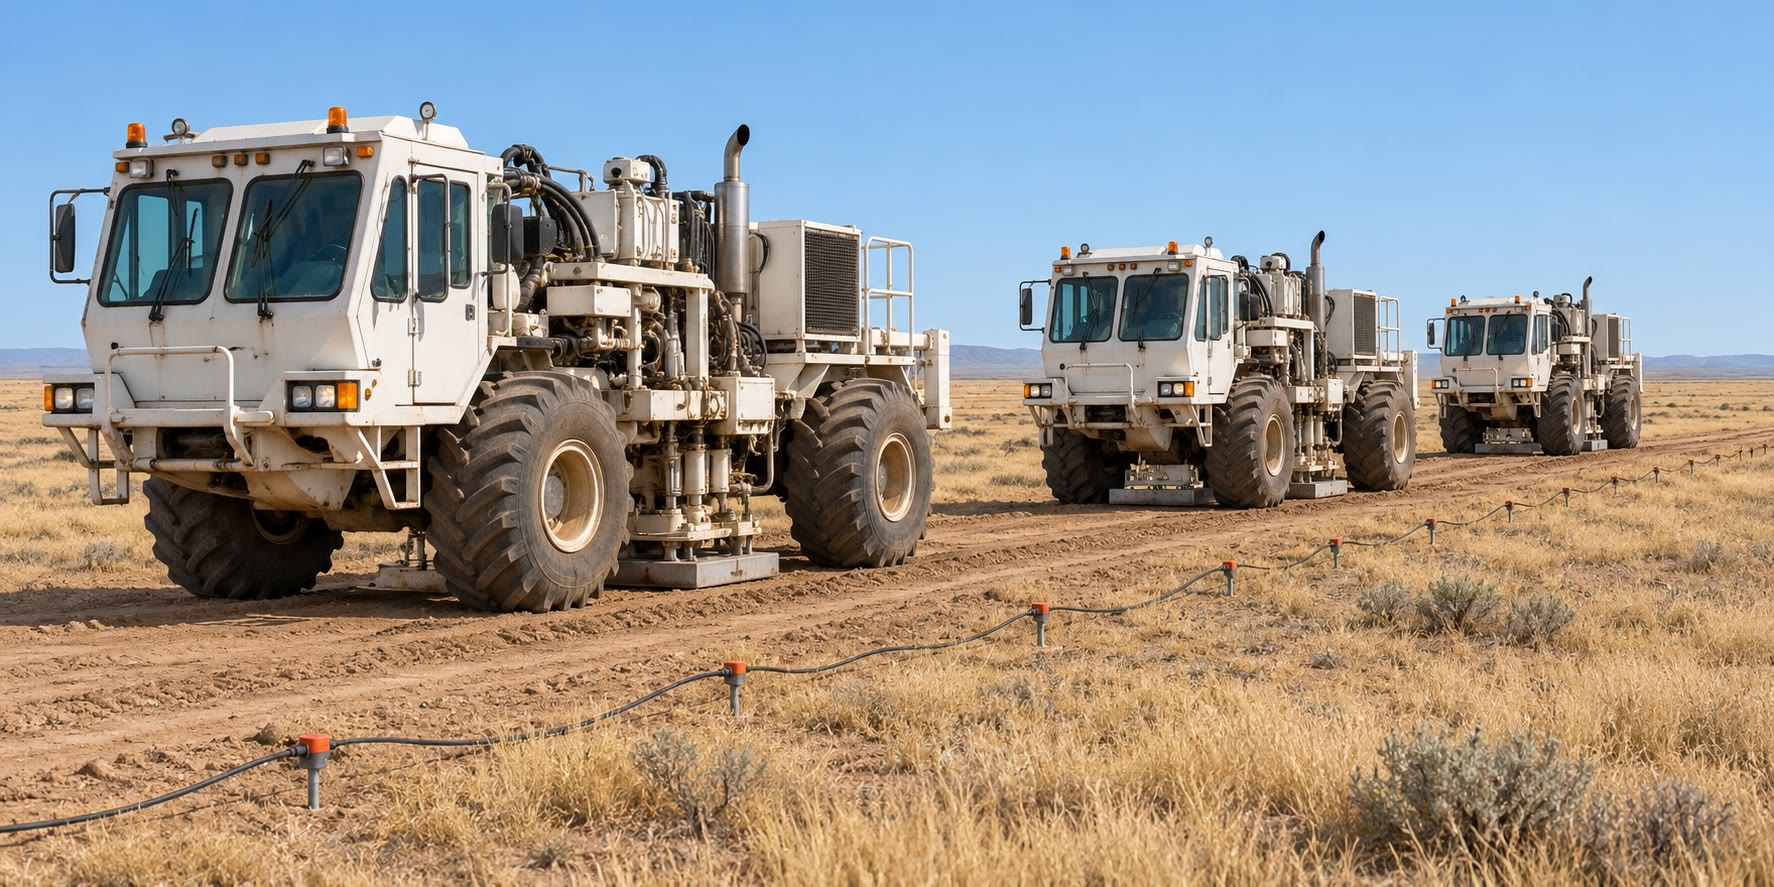
\includegraphics[width=0.62\linewidth]{images/book5/ai/b3-vibroseis.jpg}

\par\smallskip{\small شاحنات الاهتزاز على خط مسح بري: فبدلًا من الانفجار، تضغط كل شاحنة
لوحًا ثقيلًا على الأرض وتهزّها بمسح من الترددات لعدة ثوانٍ؛ وتُضغط التسجيلات الطويلة
إلى نبضات قصيرة
بإجراء الارتباط بينها وبين المسح (رسم توضيحي مولَّد بالذكاء الاصطناعي).}
\label{fig:b3:exploration-seismology:vibroseis}
\end{omfigure}

\section{الترحيل الزلزالي}

يُظهر المقطع المكدَّس كلَّ انعكاس تحت نقطة المنتصف التي سُجّل عندها،
عند الزمن الذي استغرقه للعودة. وبالنسبة إلى عاكس مستوٍ يكون ذلك في موضعه الحقيقي.
أمّا العاكس المائل فليس الأمر كذلك: فالصدى المسجَّل عند نقطة على السطح يأتي من النقطة
الأقرب إليها على العاكس، وهي تقع أعلى الانحدار، لا رأسيًا تحتها.
وتظهر نقاط مثل نهايات الصدوع، التي تبعثر الطاقة في كل الاتجاهات،
على هيئة قطوع زائدية.

\begin{definition}[الترحيل الزلزالي]\label{def:b3:exploration-seismology:migration}
\emph{الترحيل الزلزالي}\index{الترحيل الزلزالي} هي خطوة المعالجة التي
تنقل انعكاسات المقطع الزلزالي إلى مواضع العواكس التي أنتجتها، فتُستعاد الانحدارات الحقيقية
ومواضع العواكس المائلة، وتنضغط قطوع الانحراف الزائدية للمبعثرات النقطية
على قممها. وعند إجرائه بنموذج سرعة بدلالة الزمن، ينتج مقطعًا مُرحَّلًا زمنيًا؛
وبنموذج بدلالة العمق،
فالناتج صورة عمقية.
\end{definition}

\begin{theorem}[الانحدار على مقطع الإزاحة الصفرية]\label{thm:b3:exploration-seismology:dip}
في وسط سرعته $v$، يظهر عاكس مستوٍ انحداره $\theta$ في مستوى المقطع
على مقطع الإزاحة الصفرية، مرسومًا بالعمق $vt/2$ رأسيًا تحت كل نقطة تسجيل،
على هيئة خط ذي انحدار ظاهري $\theta_a$ يحقّق
العلاقة
\[
  \tan\theta_a = \sin\theta .
\]
ينشأ الانعكاس المسجَّل عند النقطة $x$ من نقطة على العاكس تبعد
مسافة $(vt/2)\sin\theta$ أعلى الانحدار من النقطة الواقعة رأسيًا تحت $x$.
\end{theorem}

\begin{proof}
الشعاع ذو الإزاحة الصفرية عمودي على العاكس، فالزمن المسجَّل عند $x$
هو $t = 2d(x)/v$، حيث $d(x)$ هي المسافة من $x$ إلى المستوى. وتزداد هذه المسافة
بمقدار $\sin\theta$ لكل وحدة من $x$ في اتجاه الانحدار، فالعمق المرسوم
العمق $vt/2 = d(x)$ ميلُه $\sin\theta$. وتقع قدم العمود الساقط من $x$
على المستوى على بُعد أفقي $d\sin\theta$ من $x$،
في الجهة الواقعة أعلى الانحدار.
\end{proof}

بما أنّ $\tan\theta_a = \sin\theta < \tan\theta$، فإنّ المقطع غير المُرحَّل يُظهر دائمًا
انحدارات أقلّ شدّةً من الانحدارات الحقيقية، ولا يُظهر انحدارات أشدّ من
\ang{45} أبدًا. وتعود النقطة المبعثرة على عمق $z$ تحت النقطة $x_0$ إلى الموضع $x$
بزمن الإزاحة الصفرية $t(x) = (2/v)\sqrt{z^2 + (x - x_0)^2}$: قطعٌ زائدي رأسه
فوق النقطة، وهو الانعراج. والترحيل في أبسط صوره، أي تكديس الانعراج،
يجمع كل مقطع على امتداد قطع الانعراج الزائدي لكل مبعثِر ممكن،
ويضع المجموع عند الرأس. فالعواكس، وهي خطوط متصلة من المبعثرات،
تظهر في مواضعها الحقيقية،
وتنضغط الانعراجات.

\begin{omfigure}
\begin{tikzpicture}[font=\small, x=1cm, y=1cm]
\draw[thick] (-0.5,0) -- (8.5,0) node[right] {سطح};
% true reflector, dip 35 deg, rising to the left
\draw[very thick, brown!70!black] (1.0,-1.2) -- (6.0,-4.70);
\node[brown!50!black, anchor=east] at (0.95,-1.2) {عاكس حقيقي};
% zero-offset normal rays from x = 2, 4, 6
\foreach \x in {2.5, 4.5, 6.5} {
  % distance from (x,0) to the line through (1,-1.2) dir (cos35,-sin35): normal n=(sin35,cos35)
  \pgfmathsetmacro{\dd}{abs(0.5736*(\x-1.0) + 0.8192*(0+1.2))}
  \draw[blue!60!black, ->] (\x,0) -- ++({-0.5736*\dd},{-0.8192*\dd});
  \fill[blue!70!black] (\x,{-\dd}) circle (1.8pt);
}
% apparent reflector through the plotted points
\pgfmathsetmacro{\da}{abs(0.5736*1.5 + 0.8192*1.2)}
\pgfmathsetmacro{\db}{abs(0.5736*5.5 + 0.8192*1.2)}
\draw[blue!70!black, thick, densely dashed] (2.5,{-\da}) -- (6.5,{-\db});
\node[blue!60!black, anchor=west] at (6.6,{-\db}) {غير مرحَّل};
\node[anchor=south, font=\scriptsize] at (4.5,0.05) {نقاط التسجيل};
\draw[->, red!70!black, thick] (6.4,{-\db+0.05}) to[bend right=25] ({6.5-0.5736*\db+0.05},{-0.8192*\db-0.12});
\end{tikzpicture}

\par\smallskip{\small ترحيل عاكس مائل (تخطيطي، الانحدار الحقيقي
\ang{35}). الشعاع ذو الإزاحة الصفرية عند كل نقطة تسجيل عمودي على
العاكس، لذا يأتي صداه من جهة الانحدار الصاعدة؛ ويُرسم رأسيًا تحت النقطة،
على العمق $vt/2$، يبدو الانعكاس أقلّ شدّةً (المتقطّع: $\tan\theta_a =
\sin\theta$، وهنا \ang{29.8})، ومُزاح نحو جهة الانحدار الهابطة. ويعيده الترحيل (السهم الأحمر) إلى موضعه.}
\label{fig:b3:exploration-seismology:migration}
\end{omfigure}

\section{الستراتيغرافيا الزلزالية}

يمثّل المقطع المُرحَّل صورةً للطبقية، ويمكن قراءته
بوصفه ستراتيغرافيا: تتبع الانعكاسات أسطح التطبّق، وهي
خطوطٌ زمنية، فهندستها تسجّل كيف امتلأ الحوض.

\begin{definition}[الستراتيغرافيا الزلزالية، السحنة الزلزالية]\label{def:b3:exploration-seismology:seismic-stratigraphy}
\emph{الستراتيغرافيا الزلزالية}\index{الستراتيغرافيا الزلزالية} هي تفسير
ستراتيغرافيا الحوض وتاريخه الترسيبي استنادًا إلى هندسة
انعكاساته الزلزالية. أمّا \emph{السحنة الزلزالية}\index{السحنة الزلزالية} فهي وحدة ثلاثية الأبعاد من الانعكاسات
تتّسم خصائصها (الاستمرارية، والسعة،
والتردّد، والهندسة الداخلية: متوازية، متباعدة، سينية، فوضوية، تلّية)
وتختلف عن خصائص جاراتها، ويُفسَّر على أنّها بيئة
ترسيبية.
\end{definition}

\begin{definition}[انقطاع العاكس]\label{def:b3:exploration-seismology:terminations}
\emph{انقطاع العاكس}\index{انقطاع العاكس} هو نهاية انعكاسٍ عند
انعكاسٍ آخر. \emph{التراكب الصاعد}\index{التراكب الصاعد}: انعكاسٌ أفقيٌّ في الأصل
ينتهي عند سطحٍ يرتفع بانحدارٍ أشدّ، فتتراكب الطبقات الأحدث
فوق منحدرٍ أقدم. \emph{التراكب الهابط}\index{التراكب الهابط}: انعكاسٌ مائل
ينتهي نحو جهة الانحدار الهابطة عند سطحٍ أقلّ شدّةً، إذ تستقرّ أطراف الطبقات المتقدّمة
على قاع الحوض. \emph{التراكب القمّي}\index{التراكب القمّي}: انعكاساتٌ مائلة
تنتهي نحو جهة الانحدار الصاعدة عند سطحٍ يعلوها، مع تعرية قليلة، إذ تلتقي قمم الطبقات المتقدّمة
بمستوى سطح البحر. \emph{البتر
الحتّي}\index{البتر الحتّي}: انعكاساتٌ تنتهي نحو جهة الانحدار الصاعدة عند
سطحٍ يعلوها ويقطعها، أي عدم التوافق.
\end{definition}

\begin{omfigure}
\begin{tikzpicture}[font=\scriptsize, x=1cm, y=1cm]
% erosional truncation: tilted beds cut by an unconformity
\begin{scope}
\foreach \k in {0,...,5} {\draw[gray!60!black] (0,{-2.3+0.32*\k}) -- (3.0,{-1.4+0.32*\k-0.25*0});}
\fill[white] (0,-0.25) -- (3.2,-0.25) -- (3.2,0.4) -- (0,0.4) -- cycle;
\draw[very thick, red!70!black] (0,-0.25) -- (3.0,-0.25);
\foreach \k in {0,1} {\draw[gray!60!black] (0,{-0.05+0.2*\k}) -- (3.0,{-0.05+0.2*\k});}
\node[anchor=north] at (1.5,-2.45) {\foreignlanguage{arabic}{(أ) البتر الحتّي}};
\end{scope}
% onlap
\begin{scope}[xshift=3.8cm]
\draw[very thick, red!70!black] (0,-2.3) -- (3.0,-0.2);
\foreach \k in {0,...,5} {\pgfmathsetmacro{\y}{-2.1+0.33*\k} \pgfmathsetmacro{\xe}{(\y+2.3)/0.7} \draw[gray!60!black] (\xe,\y) -- (3.0,\y);}
\node[anchor=north] at (1.5,-2.45) {\foreignlanguage{arabic}{(ب) التراكب الصاعد}};
\end{scope}
% downlap and toplap: clinoforms
\begin{scope}[xshift=7.6cm]
\draw[very thick, red!70!black] (0,-2.2) -- (3.6,-2.2);
\draw[very thick, blue!60!black] (0,-0.3) -- (3.6,-0.3);
\foreach \k in {0,...,5} {\draw[gray!60!black] ({0.2+0.5*\k},-0.3) .. controls ({0.7+0.5*\k},-0.4) and ({0.6+0.5*\k},-2.1) .. ({1.1+0.5*\k},-2.2);}
\node[anchor=north] at (1.8,-2.45) {\foreignlanguage{arabic}{(ج) التراكب القمّي (القمّة)، والتراكب الهابط (القاعدة)}};
\end{scope}
\end{tikzpicture}

\par\smallskip{\small انقطاعات العاكس (مقاطع تخطيطية، انعكاسات رمادية،
أسطح منتهية ملوّنة). (أ) انعكاسات مائلة تقطعها
عدم التوافق. (ب) انعكاسات أفقية تنتهي عند منحدرٍ أقدم. (ج) طبقات مائلة
لإسفينٍ متقدّمٍ نحو البحر، تنتهي نحو جهة الانحدار الصاعدة عند السطح الذي يعلوه (\omterm{def:b3:exploration-seismology:terminations}{التراكب القمّي})
ونحو جهة الانحدار الهابطة على قاع الحوض (\omterm{def:b3:exploration-seismology:terminations}{التراكب الهابط}).}
\label{fig:b3:exploration-seismology:terminations}
\end{omfigure}

تحدّد الانقطاعات الأسطحَ التي تحصر متتابعاتٍ من طبقاتٍ مترابطةٍ في أصلها
طبقاتٍ؛ ورسمُها عبر الحوض وربطُها بارتفاع مستوى البحر النسبي وانخفاضه
هو الستراتيغرافيا التتابعية، موضوعُ
\cref{ch:b3:sequence-stratigraphy}. ويُظهر المقطع الزلزالي لحافةٍ سلبيةٍ
عادةً أسافينَ من انعكاساتٍ متقدّمةٍ نحو البحر تتراكب هابطةً فوق
القاع العميق، يعلوها \omterm{def:b3:exploration-seismology:terminations}{التراكب القمّي}، وتُدفن نحو اليابسة تحت طبقاتٍ تتراكب صاعدةً
رُسِّبت حين ارتفع البحر من جديد.

\begin{inthefield}[مسحٌ بحريٌّ بالكابلات المجرورة وفريقٌ بريّ]
\begin{minipage}[t]{0.55\linewidth}\vspace{0pt}
في المسح البحري لا تتوقّف السفينة أبدًا: تُبحر خطًّا بعد خطٍّ بسرعة بضع عُقَد،
وتُطلق مصفوفاتُ المدافع الهوائية على فترات ثابتة، وتُثبَّت الكابلات المجرورة على عمقٍ
ثابتٍ بأجنحةٍ صغيرةٍ قابلةٍ للتوجيه، ويُحدَّد موقعها بالتموضع الصوتي
والساتلي. ويراقب المراقبون على الجسر البحرَ المحيطَ بالمصفوفة، ويجري المسح
وفق قواعدَ تحدّد تدابيرَ حماية الثدييات البحرية، والمراقبةَ الواجبَ إجراؤها
وما يُبلَّغ عنه.
% ledger: noaa5:itr-gom
أمّا في البرّ فيمدّ الفريق الكابلات أو وحدات التسجيل اللاسلكية على امتداد الخطوط؛
تتقدّم شاحنات الاهتزاز في قافلةٍ من نقطة مصدرٍ إلى التي تليها، وتتفقّد شاحنة
التسجيل كلّ قناةٍ قبل كلّ مسحٍ اهتزازي. وفي مركز المعالجة
تُرتَّب التسجيلات في تجمّعات \omterm{def:b3:exploration-seismology:cmp}{نقطة المنتصف المشتركة}، وتُحدَّد السرعات
ثم تُكدَّس البيانات وتُرحَّل، ويُسلَّم المقطع إلى
المفسِّرين.
\end{minipage}\hfill
\begin{minipage}[t]{0.42\linewidth}\vspace{0pt}
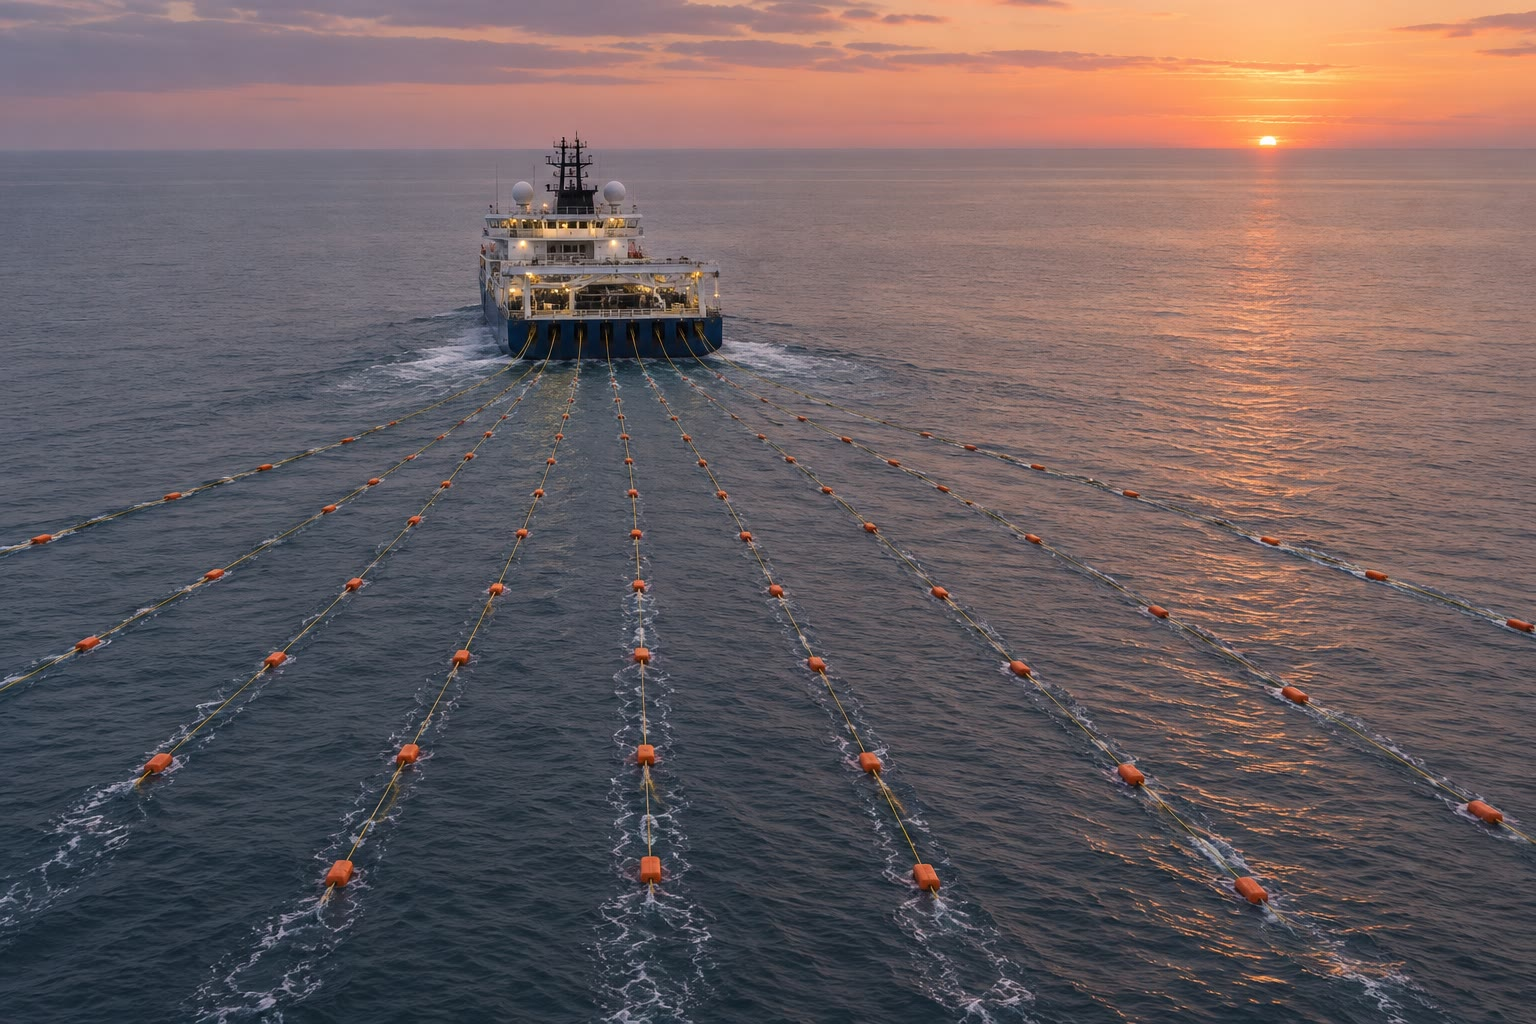
\includegraphics[width=\linewidth]{images/book5/ai/b3-streamer-vessel.jpg}

{\scriptsize سفينة مسح زلزالي تجرّ كابلاتها عند الغروب
(رسم توضيحي مولَّد بالذكاء الاصطناعي).}
\end{minipage}
\end{inthefield}

\section{التمارين}

\begin{exercise}[$\star$]\label{exo:b3:exploration-seismology:1}
الطباشير ($v = \qty{2500}{m.s^{-1}}$، $\rho = \qty{2.00}{g.cm^{-3}}$) يقع فوق
الطَّفل، سرعته \qty{2300}{m.s^{-1}} وكثافته \qty{2.30}{g.cm^{-3}}، الذي يقع فوق الحجر الجيري
سرعته \qty{4500}{m.s^{-1}} وكثافته \qty{2.60}{g.cm^{-3}}. احسب المعاوقات الصوتية الثلاث،
ومعاملات الانعكاس للسطحين البينيين. ما الجزء من الطاقة الساقطة
الذي يعكسه أعلى الحجر الجيري؟
% ledger: mavko:velocities
\end{exercise}

\begin{exercise}[$\star$]\label{exo:b3:exploration-seismology:2}
يقع عاكسٌ مستوٍ على عمق \qty{800}{m} تحت طبقةٍ سرعتها \qty{2000}{m.s^{-1}}.
احسب $t_0$، زمن الانعكاس عند إزاحةٍ قدرها \qty{1000}{m}، \omterm{thm:b3:exploration-seismology:nmo}{والانزياح الزمني العادي}
عند تلك الإزاحة. قارن النتيجة بالتقريب $x^2/(2v^2t_0)$.
\end{exercise}

\begin{exercise}[$\star$]\label{exo:b3:exploration-seismology:3}
يحتوي الكابل على 240 قناةً تتباعد \qty{12.5}{m}، وتُطلق السفينة كلّ
\qty{25}{m}. احسب فاصل \omterm{def:b3:exploration-seismology:cmp}{نقطة المنتصف المشتركة} \omterm{def:b3:exploration-seismology:cmp}{وتعدّدية التغطية}. ما فاصل الإطلاق الذي
يعطي تعدّدية تغطية قدرها 120؟
\end{exercise}

\begin{exercise}[$\star$]\label{exo:b3:exploration-seismology:4}
عند تردّد سائد قدره \qty{30}{Hz}، احسب طول الموجة
وربع طول الموجة في الحجر الرملي ذي السرعة \qty{3000}{m.s^{-1}} وفي الحجر الجيري ذي
السرعة \qty{4500}{m.s^{-1}}. احسب نصف قطر \omterm{def:b3:exploration-seismology:fresnel}{نطاق فرينل} الأول لعاكسٍ على
عمق \qty{1000}{m} تحت صخور متوسط سرعتها \qty{2800}{m.s^{-1}}.
\end{exercise}

\begin{exercise}[$\star\star$]\label{exo:b3:exploration-seismology:5}
لانعكاسين لهما $t_0 = \qty{0.500}{s}$ \omterm{def:b3:exploration-seismology:velocities}{وسرعة الجذر التربيعي للمتوسط} قدرها
\qty{2400}{m.s^{-1}}، ولانعكاس آخر $t_0 = \qty{0.700}{s}$ وسرعته \qty{2800}{m.s^{-1}}.
احسب \omterm{def:b3:exploration-seismology:velocities}{السرعة الفاصلية} وسمك الطبقة الواقعة بينهما.
\end{exercise}

\begin{exercise}[$\star\star$]\label{exo:b3:exploration-seismology:6}
ينحدر عاكسٌ مستوٍ بزاوية $\varphi$ في مستوى خطّ \omterm{def:b3:exploration-seismology:cmp}{نقطة المنتصف المشتركة}، ضمن طبقةٍ
سرعتها $v$. (أ) بيّن أنّ $t(x)^2 = t_0^2 + x^2\cos^2\varphi/v^2$، حيث $t_0$ هو
زمن الإزاحة الصفرية عند نقطة المنتصف. (تلميح: استخدم صورة نقطة المنتصف في
العاكس.) (ب) استنتج \omterm{def:b3:exploration-seismology:velocities}{سرعة التكديس}، واحسبها من أجل
$v = \qty{2000}{m.s^{-1}}$ و$\varphi = \ang{12}$.
\end{exercise}

\begin{exercise}[$\star\star$]\label{exo:b3:exploration-seismology:7}
تحتوي مجموعةٌ ذات تعدّدية تغطية 60 على ضوضاءٍ مستقلّة ذات تباينٍ متساوٍ في كلّ أثرٍ. بأيّ عاملٍ
يرفع \omterm{def:b3:exploration-seismology:stack}{التكديس} نسبة الإشارة إلى الضوضاء؟ وبأيّ عاملٍ يجب أن تُزاد
\omterm{def:b3:exploration-seismology:cmp}{تعدّدية التغطية} لمضاعفتها مرّةً أخرى؟
\end{exercise}

\begin{exercise}[$\star\star$]\label{exo:b3:exploration-seismology:8}
على مقطع زمن الإزاحة الصفرية، في صخورٍ سرعتها \qty{3000}{m.s^{-1}}، يرتفع انعكاسٌ
بمقدار \qty{0.40}{s} من زمن الذهاب والإياب لكلّ كيلومتر على طول الخطّ. حوّل هذا
الميل إلى انحدارٍ ظاهريّ، واحسب الانحدار الحقيقي للعاكس.
\end{exercise}

\begin{exercise}[$\star\star$]\label{exo:b3:exploration-seismology:9}
احسب التفاف \omterm{def:b3:exploration-seismology:synthetic}{متسلسلة الانعكاسية} $r = (0, 0.3, 0, -0.2, 0)$ مع
\omterm{def:b3:exploration-seismology:wavelet}{الموجة الزلزالية القصيرة} ذات ثلاث عيّنات $w = (-0.5, 1, -0.5)$، عيّنةً بعيّنة. أين يقع
الانعكاسان، وهل يتداخلان؟
\end{exercise}

\begin{exercise}[$\star\star\star$]\label{exo:b3:exploration-seismology:10}
يُعطي مقطع الانكسار المعكوس فوق طبقةٍ سرعتها \qty{1800}{m.s^{-1}} سرعةً ظاهريةً
نحو الانحدار قدرها \qty{2900}{m.s^{-1}}، وأخرى عكس الانحدار قدرها
\qty{4400}{m.s^{-1}}. احسب زاوية الحرج والانحدار وسرعة
السطح الانكساري. قارن سرعة السطح الانكساري بالمتوسط التوافقي للسرعتين
الظاهريّتين.
\end{exercise}

\begin{exercise}[$\star\star\star$]\label{exo:b3:exploration-seismology:11}
في \cref{prop:b3:exploration-seismology:tuning}، لطبقةٍ
معاملا انعكاسٍ $+R$ و$-R$. (أ) بيّن أنّ الإشارة المركّبة، من أجل $\Delta t \ll T$،
تساوي تقريبًا $R\,\Delta t\,w'(t)$، أي المشتقّة الزمنية للموجة القصيرة
مضروبةً في سمك الطبقة ذهابًا وإيابًا. (ب) فسّر لماذا يمكن أن تُكشف طبقةٌ رقيقة
وإن لم تُفصَل، وكيف يمكن تقدير سمكها من
سعتها. (ج) لطبقتين من الصخر نفسه، سمكهما 5 و\qty{10}{m}، تُصوَّران
بالموجة القصيرة نفسها: ما نسبة سعتيهما؟
\end{exercise}

\begin{exercise}[$\star\star\star$]\label{exo:b3:exploration-seismology:12}
يقع مبعثِر نقطي على بعد \qty{600}{m} تحت الخطّ، في صخورٍ
سرعتها \qty{3000}{m.s^{-1}}. (أ) اكتب زمن الإزاحة الصفرية لحيودها بدلالة
المسافة الأفقية $x$ عن النقطة الواقعة فوقه، واحسبه عند $x = 0$
و\qty{300}{m}. (ب) بيّن أنّ الحيود قطعٌ زائد من صيغة NMO
بالسرعة $v/2$، وفسّر لماذا يكون الحيود دائمًا أشدّ انحناءً من
انعكاسٍ له زمن القمّة نفسه. (ج) ما أثر الترحيل فيه؟
\end{exercise}

\section{مسألة: خطّ زلزالي عبر تلال فاردن}

\begin{problem}[{مسألة نهاية الأسبوع --- الانكسار وتحليل السرعة والتحويل إلى
العمق والترحيل على المقطع A--B لتلال فاردن}]
\label{pb:b3:exploration-seismology:1}
% values: calc/ch02.py, from figdata seismic_model.py, refraction_dip.py, cmp_nmo.py
يُطلق خطٌّ زلزالي على طول المقطع A--B لتلال فاردن، المنطقة
الواردة في الخرائط الجيولوجية للمجلدات السابقة. تُحسب مسافاته $s$ انطلاقًا من
A على طول الخطّ. يتألّف الغطاء الرسوبي، من الأعلى، من الطباشير والطَّفل (\qty{100}{m})،
الحجر الجيري (\qty{180}{m}) والحجر الرملي (\qty{120}{m})، يرقد بعدم توافق على
قاعدةٍ من الشيست؛ وهو مطويّ في طيّةٍ محدّبة وأخرى مقعّرة، ومقطوعٌ بصدعٍ
عادي.

\medskip
\noindent\textbf{الجزء الأول --- مسحٌ انكساري على الجناح الغربي.} يُقام مسحٌ بطول
\qty{1200}{m} بين نقطتي الإطلاق \babelsublr{W ($s = \qty{300}{m}$)}
و\babelsublr{E ($s = \qty{1500}{m}$)}، على أرضٍ تُعدّ مستويةً. تُعامل الطباشير والطَّفل
الواقعَين فوق الحجر الجيري طبقةً واحدةً ذات $v_1 = \qty{2.40}{km.s^{-1}}$. وتُقرأ أزمنة
موجة الرأس المقروءة على التسجيلات هي، من W نحو E، \qty{425.2}{ms} عند
\qty{800}{m} و\qty{486.1}{ms} عند \qty{1200}{m}؛ ومن E نحو W،
\qty{372.4}{ms} عند \qty{800}{m} و\qty{486.1}{ms} عند \qty{1200}{m}.
\begin{enumerate}
  \item احسب السرعتين الظاهريّتين. أيّ الإطلاقين عكس الانحدار؟
  \item احسب زاوية الحرج وانحدار السطح الانكساري.
  \item احسب سرعة السطح الانكساري. أيّ صخرٍ هو؟
  \item احسب أزمنة التقاطع والأعماق العمودية للسطح
        الانكساري تحت W وتحت E.
  \item حوّل هذه الأعماق إلى أعماقٍ رأسية، وتحقّق من الانحدار انطلاقًا من العمقين.
  \item الطَّفل الواقع تحت الطباشير أبطأ من الطباشير. ما الذي يستنتجه
        مسح الانكسار منه، وكيف يُحدث انحيازًا في الأعماق؟
\end{enumerate}

\noindent\textbf{الجزء الثاني --- تحليل السرعة عند \omterm{def:b3:exploration-seismology:cmp}{نقطة المنتصف المشتركة} S.} أبعد نحو الشرق، \omterm{def:b3:exploration-seismology:cmp}{نقطة المنتصف المشتركة} S
تقع على محور الطية المقعرة، في الكتلة الهابطة من الصدع، حيث
تُعتبر الطبقات مستوية. تُلتقط أربعة انعكاسات عند الإزاحة الصفرية وعند
\qty{600}{m}:
\begin{center}
\small
\begin{tabular}{lcccc}
الانعكاس & 1 & 2 & 3 & 4 \\
الانعكاس & 1 & 2 & 3 & 4 \\
\mbox{\textdir TLT $t_0$ (\unit{s})} & 0.4878 & 0.5748 & 0.6548 & 0.7348 \\
\mbox{\textdir TLT $t(\qty{600}{m})$ (\unit{s})} & 0.5437 & 0.6240 & 0.6887 & 0.7648 \\
\hline
\end{tabular}
\end{center}
\begin{enumerate}[resume]
  \item احسب سرعة الانزياح العادي $V = x/\sqrt{t^2 - t_0^2}$ للانعكاسين 1
        و2. لماذا تكون الثانية أصغر من الأولى؟
  \item احسبها للانعكاسين 3 و4.
  \item بأخذ هذه السرعات على أنها سرعات الجذر التربيعي للمتوسط، احسب \omterm{def:b3:exploration-seismology:velocities}{السرعة الفاصلية} لكل
        طبقة \omterm{thm:b3:exploration-seismology:dix}{بمعادلة ديكس}.
  \item حدّد الطبقات من سرعاتها، وسمِّ السطوح العاكسة
        الأربعة.
  \item الانعكاس 1 هو الأضعف في التسجيلات. لماذا؟
  \item لماذا قيست السرعات على الإزاحات حتى \qty{600}{m}
        فقط، في حين أنّ الانتشار يبلغ \qty{2}{km}؟
\end{enumerate}

\noindent\textbf{الجزء الثالث --- تحويل الأعماق والتفريق.}
\begin{enumerate}[resume]
  \item احسب زمن الذهاب والإياب في كل طبقة وسمكها.
  \item احسب عمق كل سطح عاكس تحت سطح الأرض. قارن
        أسماك الطَّفل والحجر الجيري والحجر الرملي بالقيم المعطاة
        أعلاه.
  \item احسب متوسط السرعة من سطح الأرض حتى القاعدة، وفسّر لماذا
        ستبالغ سرعة الانزياح العادي للانعكاس 4 في تقدير العمق إذا استُخدمت
        بدلًا منها.
  \item موجة المسح الذروية عند \qty{30}{Hz}. احسب طول الموجة في
        الطَّفل \omterm{def:b3:exploration-seismology:resolution}{وسمك التوليف} له، سواء بقاعدة ربع الطول الموجي
        أم بالعلاقة $b = v/(5.2f)$ \omterm{def:b3:exploration-seismology:wavelet}{لموجة ريكر القصيرة}. هل يُفرَّق الطَّفل؟
        عند أيّ تردّد يحدث التوليف بقاعدة ربع الطول الموجي؟
  \item احسب نصف قطر \omterm{def:b3:exploration-seismology:fresnel}{نطاق فرينل} الأول على القاعدة، مع أخذ
        $\lambda$ من سرعة الانزياح العادي للانعكاس 4.
\end{enumerate}

\noindent\textbf{الجزء الرابع --- الهجرة والصدع.}
\begin{enumerate}[resume]
  \item قرب الصدع، ينتج عن قطع الحجر الجيري حيودٌ
        قمّته عند \qty{0.550}{s}؛ وعلى بعد \qty{200}{m} من القمّة على الخط
        نفسه يكون عند \qty{0.5732}{s}. اكتب زمن الحيود عند الإزاحة الصفرية،
        واستنتج متوسط السرعة فوق القطع.
  \item احسب عمق القطع تحت سطح الأرض.
  \item على الجناح الشرقي، يرتفع انعكاس أعلى الحجر الجيري في المقطع المكدّس
        نحو الطية المحدبة بمقدار \qty{0.167}{s} من زمن الذهاب والإياب لكل
        كيلومتر، تحت صخور متوسط سرعتها \qty{2.48}{km.s^{-1}}. احسب انحداره
        الظاهري وانحداره الحقيقي.
  \item يُسجَّل انعكاس على ذلك الجناح عند $t = \qty{0.655}{s}$. ما مقدار
        الانتقال الذي تُحدثه الهجرة فيه، وفي أيّ اتجاه؟
  \item عبر الصدع يقفز انعكاس القاعدة العلوي بمقدار \qty{0.160}{s}؛
        والكتلة الهابطة تحمل السمك الإضافي في الطباشير. احسب
        مقدار الإزاحة.
  \item أعطِ عمق عدم التوافق القاعدي تحت \omterm{def:b3:exploration-seismology:cmp}{نقطة المنتصف المشتركة} S، انطلاقًا من
        السرعات الفاصلية للجزء الثاني.
\end{enumerate}
\end{problem}
